
\section{光储充电站系统暂态稳定性仿真分析}

在第二章完成光储充电站各关键物理单元数学建模与控制策略设计的基础上，本章旨在通过 MATLAB/Simulink 时域电磁暂态仿真，全面验证系统在多重极端扰动下的暂态稳定性。根据实际运行工况与课题要求，微电网的暂态稳定性主要面临三大核心扰动源：自然环境突变导致的光伏出力剧烈变化（源侧扰动）、大型充电负荷的突然启动与切除（荷侧扰动），以及电网侧发生的三相短路故障（网侧扰动）。

本章首先给出了系统级仿真平台的关键参数配置；随后，针对上述三种典型暂态扰动场景分别开展了深度仿真。通过对直流母线电压、储能充放电电流、并网有功/无功功率等关键电气量的动态响应过程进行深度剖析，揭示了微电网在源网荷强耦合作用下的暂态演变机理，并重点评估了系统在极端工况下的电压稳定性。

\subsection{仿真平台搭建与关键参数配置}

为确保仿真结果的准确性与工程参考价值，本文基于 MATLAB/Simulink 软件平台，调用 Simscape Electrical 电力系统专业元件库，搭建了兆瓦级光储充电站系统级电磁暂态仿真模型。

在仿真求解器（Solver）配置方面，为兼顾暂态计算的精度与非线性电力电子器件的收敛性，系统采用 ode23tb 变步长刚性求解算法，最大仿真步长限制为 $1 \times 10^{-4}$ 秒，以确保能够精确捕捉到短路故障瞬间及开关动作产生的高频电气量突变。

光伏阵列、储能电池、并网逆变器及等效恒功率充电负荷的核心仿真参数设定如表 \ref{tab:sim_parameters} 所示。

\begin{table}[htbp]
    \centering
    \caption{光储充电站系统关键仿真参数}
    \label{tab:sim_parameters}
    \begin{tabular}{lcc}
        \toprule
        \textbf{系统模块} & \textbf{参数名称} & \textbf{数值及单位} \\
        \midrule
        \multirow{2}{*}{直流母线与电网} 
        & 直流母线额定参考电压 $V_{dc\_ref}$ & 1500 V \\
        & 交流电网线电压有效值 $E_{line}$ & 380 V \\
        & 交流电网基波频率 $f$ & 50 Hz \\
        \midrule
        \multirow{3}{*}{光伏发电系统} 
        & 光伏阵列最大输出功率 $P_{pv\_max}$ & 1.35 MW \\
        & 开路电压 $V_{oc}$ / 短路电流 $I_{sc}$ & 532.8 V / 3491.4 A \\
        & Boost 变换器开关频率 $f_{s\_pv}$ & 20 kHz \\
        \midrule
        \multirow{3}{*}{储能电池系统} 
        & 锂离子电池额定容量 $C_{bat}$ & 200 Ah \\
        & 电池标称电压 $V_{bat\_nom}$ & 1000 V \\
        & 初始荷电状态 $SOC_{init}$ & 50 \% \\
        \midrule
        \multirow{2}{*}{并网逆变器系统} 
        & LCL 滤波器网侧电感 $L_{g}$ & 9 mH \\
        & 逆变器开关频率 $f_{s\_inv}$ & 8 kHz \\
        \midrule
        \multirow{2}{*}{充电负荷(CPL)} 
        & 阶跃突加额定快充功率 $P_{cpl}$ & 200 kW \\
        & 阶跃突加时刻 $t_{step}$ & 0.3 s \\
        \bottomrule
    \end{tabular}
\end{table}

\subsection{工况一：光伏出力剧烈变化暂态响应分析（源侧扰动）}

本工况主要考察光储充电站微电网在面临自然环境突变（如乌云遮挡导致光照骤降）时，系统维持直流母线电压稳定及功率动态平衡的能力。

在仿真设置中，系统初始运行于稳态，大功率充电负荷（CPL）保持恒定功率抽取。在仿真时间 $t=0.3\text{s}$ 时，设定光伏阵列接收到的太阳辐照度发生阶跃跌落，模拟极端的源侧功率丧失扰动。系统关键电气量的暂态响应波形如图 \ref{fig:scenario1_waveforms} 所示。

\begin{figure}[htbp]
    \centering
    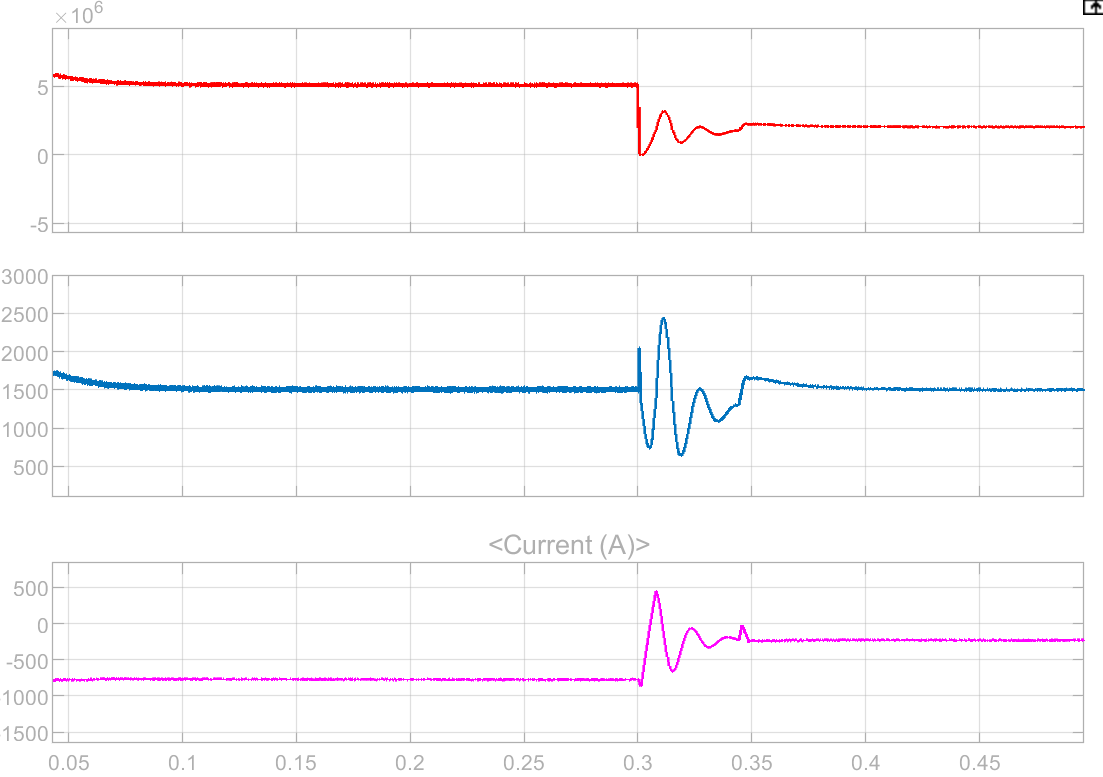
\includegraphics[width=0.85\textwidth]{figures/fig3_1_scenario1.png}
    \caption{光照骤降工况下系统关键电气量暂态波形}
    \label{fig:scenario1_waveforms}
\end{figure}

结合理论与仿真波形分析可知，在 $t=0.3\text{s}$ 光伏有功出力剧烈跌落的瞬间（如图 \ref{fig:scenario1_waveforms} 顶层波形所示），由于恒功率充电负荷（CPL）的功率需求保持不变，直流微电网内部瞬间出现了严重的功率缺额（即源侧发出的功率远小于荷侧消耗的功率）。这一极端的功率不平衡导致直流母线电容上的能量被迅速抽离，表现为中层波形中直流母线电压 $V_{dc}$ 在 $0.3\text{s}$ 处出现了明显的下凹跌落，偏离了 $1500\text{V}$ 的额定参考值。

与此同时，储能系统（ESS）的电压外环控制敏锐地捕捉到了母线电压的负向偏差（$V_{dc\_ref} - V_{dc} > 0$），并通过 PI 调节器迅速生成了极大的正向放电电流指令。由底层波形可见，电池电流在极短的毫秒级时间内，从原本的充电状态（约 $-800\text{A}$）瞬间反转并飙升至巨大的放电峰值（约 $+500\text{A}$）。在储能系统强大的瞬时功率支撑作用下，直流母线电压的跌落趋势被迅速遏制，并经过短暂的阻尼振荡后，在 $t=0.35\text{s}$ 左右重新恢复并稳定在 $1500\text{V}$ 的额定值。

上述暂态过程充分验证了本文在第二章所设计的储能双向变换器双闭环控制策略具备极高的动态响应带宽。同时，在面临源侧剧烈功率丧失的极端扰动时，系统不仅没有发生电压崩溃，反而能够依托储能单元快速建立新的全局功率平衡，证明了该直流微电网系统架构与控制参数具备优异的鲁棒性。

\subsection{工况二：大型充电负荷突然启动与切除暂态分析（荷侧扰动）}

本工况是本文暂态稳定性分析的核心环节，旨在验证当兆瓦级光储充电站面临大功率恒功率负载（CPL）瞬间切入与切除时，微电网系统克服 CPL 负阻抗特性、维持直流母线电压稳定的能力。

在仿真中，设定光照条件保持满载恒定。在 $t=0.2\text{s}$ 时，通过阶跃脉冲信号模拟大型电动汽车车队突然接入，充电桩抽取功率从 $20\text{kW}$ 的基础待机负荷瞬间跃升至 $200\text{kW}$；在 $t=0.4\text{s}$ 时，模拟充电完成或突发断开，负荷功率瞬间跌回 $20\text{kW}$。该连续大扰动工况下系统的关键电气量响应波形如图 \ref{fig:scenario2_waveforms} 所示。

\begin{figure}[htbp]
    \centering
    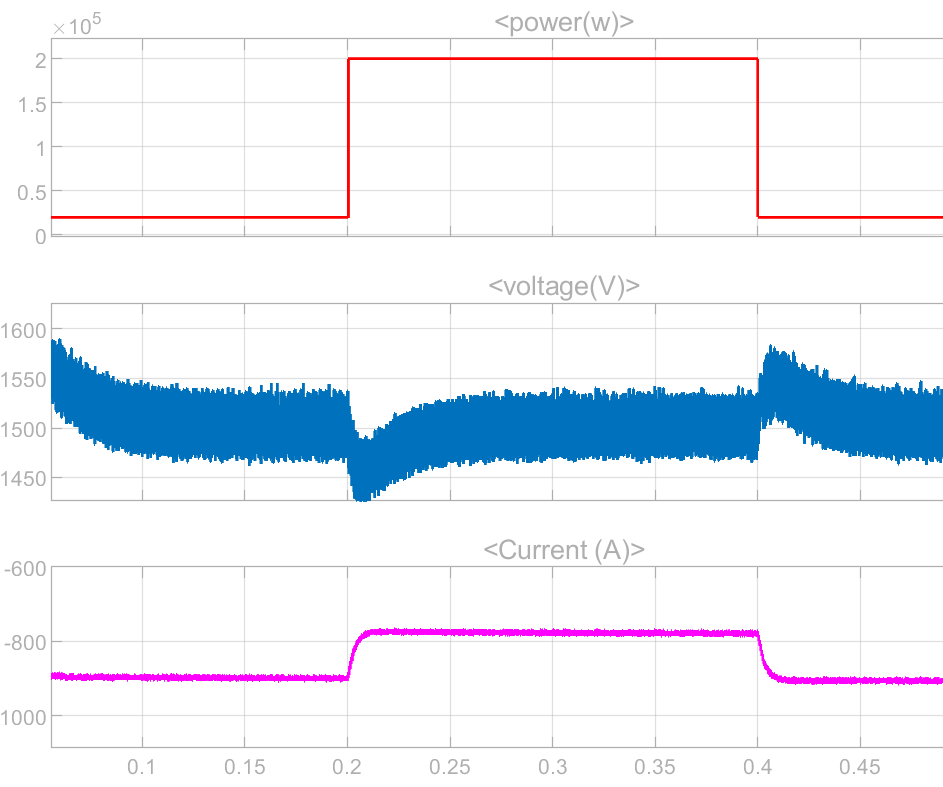
\includegraphics[width=0.85\textwidth]{figures/fig3_2_scenario2.png}
    \caption{充电负荷阶跃突加与突卸工况下暂态波形}
    \label{fig:scenario2_waveforms}
\end{figure}

观察图 \ref{fig:scenario2_waveforms} 中层的直流母线电压波形可知，由于本文采用了真实的物理开关级模型（Switching-level Model），母线电压包络线中清晰地叠加了由电力电子器件高频动作（$10\text{kHz}$）引发的开关纹波，高度还原了物理电网的真实运行状态。

在 $t=0.2\text{s}$ 负荷功率突增的瞬间，CPL 的负阻抗特性（即功率恒定、电压跌落导致抽取电流进一步增大）对母线造成了强烈的冲击，导致 $V_{dc}$ 出现陡峭的下凹跌落（最低至约 $1430\text{V}$）。此时，储能电池系统（底层波形）迅速响应，其电流从约 $-900\text{A}$（充电状态）极速攀升至 $-780\text{A}$ 左右（减少充电并向放电趋势强力拉扯），通过释放/少吸能量填补了 CPL 带来的巨大功率缺口，使母线电压在数十毫秒内重新钳位至 $1500\text{V}$。

在 $t=0.4\text{s}$ 负荷瞬间切除时，系统出现了反向的暂态过程。由于负荷瞬间消失而储能与光伏系统的功率输出存在微小的控制惯性，多余的能量瞬间涌入直流母线电容，导致 $V_{dc}$ 出现了明显的上凸过冲（最高至约 $1570\text{V}$）。储能外环电压控制器立即捕捉到过压信号，指令电流内环迅速深跌（电流变负增强），储能电池瞬间吸收了多余的激增功率，再次将母线电压平滑压制回额定稳态值。

这一完整的“跌落-恢复”与“过冲-恢复”双向暂态过程，不仅直观展示了 CPL 负阻抗特性对微电网的破坏力，更有力地证明了本文所设计的储能双闭环控制策略能够在极端的双向功率冲击下，保障光储充直流微电网的绝对稳定性。

\section{网侧三相短路故障穿越分析}

在微电网实际运行中，交流大电网侧的极端故障（如线路短路、雷击等）会对直流微电网的稳定运行造成严重冲击。本节通过模拟大电网发生三相短路故障，验证所设计的直流微电网系统在极端交流侧扰动下的暂态响应特性与故障穿越能力。

设定系统在额定工况下稳定运行（光伏输出稳定，受控源恒功率负载维持 $200\text{kW}$）。在 $t=0.3\text{s}$ 时，交流并网点（PCC）突发严重的三相对称短路故障，电网电压发生深度跌落；故障持续 $0.05\text{s}$ 后，于 $t=0.35\text{s}$ 时由断路器切除，电网恢复正常。该工况下的系统暂态波形如图 \ref{fig:scenario3} 所示。

\begin{figure}[htbp]
    \centering
    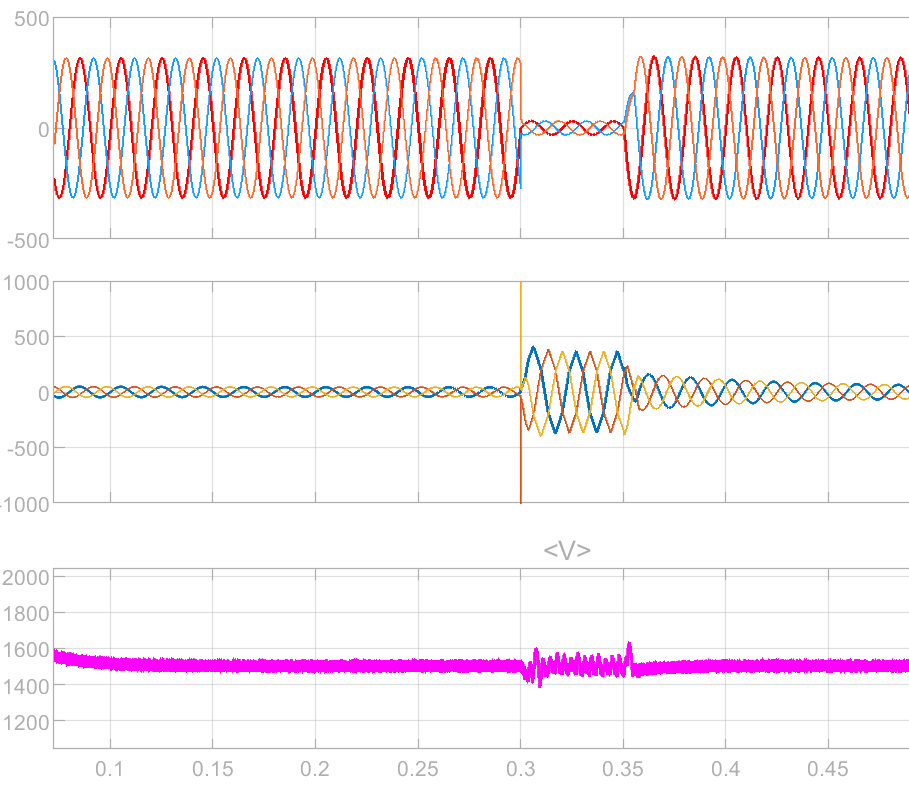
\includegraphics[width=0.85\textwidth]{figures/fig3_3_scenario3.png}
    \caption{网侧三相短路故障暂态响应波形}
    \label{fig:scenario3}
\end{figure}

由图 \ref{fig:scenario3} 的交流侧电压与电流波形可知，在 $t=0.3\text{s}$ 故障发生瞬间，PCC 点三相电压幅值骤降至接近零值。受电网电压深度跌落影响，逆变器输出功率受阻，导致网侧电流在短路瞬间出现激增现象。然而，得益于并网逆变器 PQ 控制策略中电流内环的快速限幅与调节作用，短路电流被有效抑制在安全范围内，避免了电力电子器件的过流损坏。在 $t=0.35\text{s}$ 故障切除后，网侧电压瞬间恢复至额定值，交流电流经过约 $0.05\text{s}$ 的平滑动态调整后，重新恢复至故障前的稳态并网波形，未出现控制系统的积分饱和或低频振荡发散现象。

从直流母线电压波形可以观察到，在网侧短路期间（$0.3\text{s} \sim 0.35\text{s}$），由于逆变器向交流电网输送功率的通道受阻，光伏阵列发出的有功功率在直流侧大量积压，打破了系统原有的功率平衡。这一极端的功率冲击导致直流母线电压发生高频暂态振荡。此时，蓄电池双向 Buck-Boost 变流器的电压外环迅速响应，立刻切换工作状态以吸收冗余的瞬态功率。在储能系统的强力平抑下，直流母线电压的最大波动被严格限制在 $1400\text{V} \sim 1600\text{V}$ 之间（最大偏差率低于 $6.7\%$），确保了母线电容及挂载设备的安全。在故障清除后，母线电压迅速收敛并稳定于 $1500\text{V}$ 额定值。

上述仿真结果充分证明，本文构建的直流微电网及其协调控制策略具有优异的鲁棒性。在面临大电网严重短路故障的极端工况下，系统不仅能够维持直流母线的动态稳定，还能在故障清除后迅速实现状态恢复，具备可靠的故障穿越（Fault Ride-Through）能力。
